%%%%%%%%%%%%%%%%%%%%%%%%%%%%%%%%%%%%%%%%%
% Jacobs Landscape Poster
% LaTeX Template
% Version 1.1 (14/06/14)
%
% Created by:
% Computational Physics and Biophysics Group, Jacobs University
% https://teamwork.jacobs-university.de:8443/confluence/display/CoPandBiG/LaTeX+Poster
% 
% Further modified by:
% Nathaniel Johnston (nathaniel@njohnston.ca)
%
% This template has been downloaded from:
% http://www.LaTeXTemplates.com
%
% License:
% CC BY-NC-SA 3.0 (http://creativecommons.org/licenses/by-nc-sa/3.0/)
%
%%%%%%%%%%%%%%%%%%%%%%%%%%%%%%%%%%%%%%%%%

%----------------------------------------------------------------------------------------
%	PACKAGES AND OTHER DOCUMENT CONFIGURATIONS
%----------------------------------------------------------------------------------------

\documentclass[final]{beamer}
\usepackage{bbm}
\usepackage{dsfont}
\usepackage[scale=1.24]{beamerposter} % Use the beamerposter package for laying out the poster

\usetheme{confposter} % Use the confposter theme supplied with this template

\setbeamercolor{block title}{fg=ngreen,bg=white} % Colors of the block titles
\setbeamercolor{block body}{fg=black,bg=white} % Colors of the body of blocks
\setbeamercolor{block alerted title}{fg=white,bg=dblue!70} % Colors of the highlighted block titles
\setbeamercolor{block alerted body}{fg=black,bg=dblue!10} % Colors of the body of highlighted blocks
% Many more colors are available for use in beamerthemeconfposter.sty

%-----------------------------------------------------------
% Define the column widths and overall poster size
% To set effective sepwid, onecolwid and twocolwid values, first choose how many columns you want and how much separation you want between columns
% In this template, the separation width chosen is 0.024 of the paper width and a 4-column layout
% onecolwid should therefore be (1-(# of columns+1)*sepwid)/# of columns e.g. (1-(4+1)*0.024)/4 = 0.22
% Set twocolwid to be (2*onecolwid)+sepwid = 0.464
% Set threecolwid to be (3*onecolwid)+2*sepwid = 0.708

\newlength{\sepwid}
\newlength{\onecolwid}
\newlength{\twocolwid}
\newlength{\threecolwid}
\setlength{\paperwidth}{48in} % A0 width: 46.8in
\setlength{\paperheight}{36in} % A0 height: 33.1in
\setlength{\sepwid}{0.024\paperwidth} % Separation width (white space) between columns
\setlength{\onecolwid}{0.22\paperwidth} % Width of one column
\setlength{\twocolwid}{0.464\paperwidth} % Width of two columns
\setlength{\threecolwid}{0.708\paperwidth} % Width of three columns
\setlength{\topmargin}{-0.5in} % Reduce the top margin size
%-----------------------------------------------------------

\usepackage{graphicx}  % Required for including images

\usepackage{booktabs} % Top and bottom rules for tables

%----------------------------------------------------------------------------------------
%	TITLE SECTION 
%----------------------------------------------------------------------------------------

\title{2014 World Cup Recap} % Poster title

\author{Weichen Ning, Wen Bo} % Author(s)

\institute{Department of ECE, Duke University} % Institution(s)

%----------------------------------------------------------------------------------------

\begin{document}

\addtobeamertemplate{block end}{}{\vspace*{2ex}} % White space under blocks
\addtobeamertemplate{block alerted end}{}{\vspace*{2ex}} % White space under highlighted (alert) blocks

\setlength{\belowcaptionskip}{2ex} % White space under figures
\setlength\belowdisplayshortskip{2ex} % White space under equations

\begin{frame}[t] % The whole poster is enclosed in one beamer frame

\begin{columns}[t] % The whole poster consists of three major columns, the second of which is split into two columns twice - the [t] option aligns each column's content to the top

\begin{column}{\sepwid}\end{column} % Empty spacer column

\begin{column}{\onecolwid} % The first column

%----------------------------------------------------------------------------------------
%	OBJECTIVES
%----------------------------------------------------------------------------------------

\begin{alertblock}{Objectives}

We want to apply our machine learning knowledge to real world application of world cup.
\begin{itemize}
\item Be able to formulate machine learning problems corresponding to specific application.
\item Understand the basic theory underlying machine learning.
\item Understand a range of machine learning algorithms.
\item  Be able to apply machine learning algorithms to solve problems. 
\end{itemize}

\end{alertblock}

%----------------------------------------------------------------------------------------
%	INTRODUCTION
%----------------------------------------------------------------------------------------

\begin{block}{Introduction}

We develop a Bayesian approach to predict the 2014 FIFA World Cup (especially focus on elimination games), by applying probit regression and Bayesian linear regression model with data augmentation. For our model, we develop the Gibbs sampler to perform the posterior inference. We apply our algorithms on the different datasets and the results show that we could obtain high accurate predictions.

\end{block}

%------------------------------------------------
\begin{figure}
\includegraphics[width=0.8\linewidth]{graph.jpg}
\caption{Graphical Model}
\end{figure}

\begin{figure}
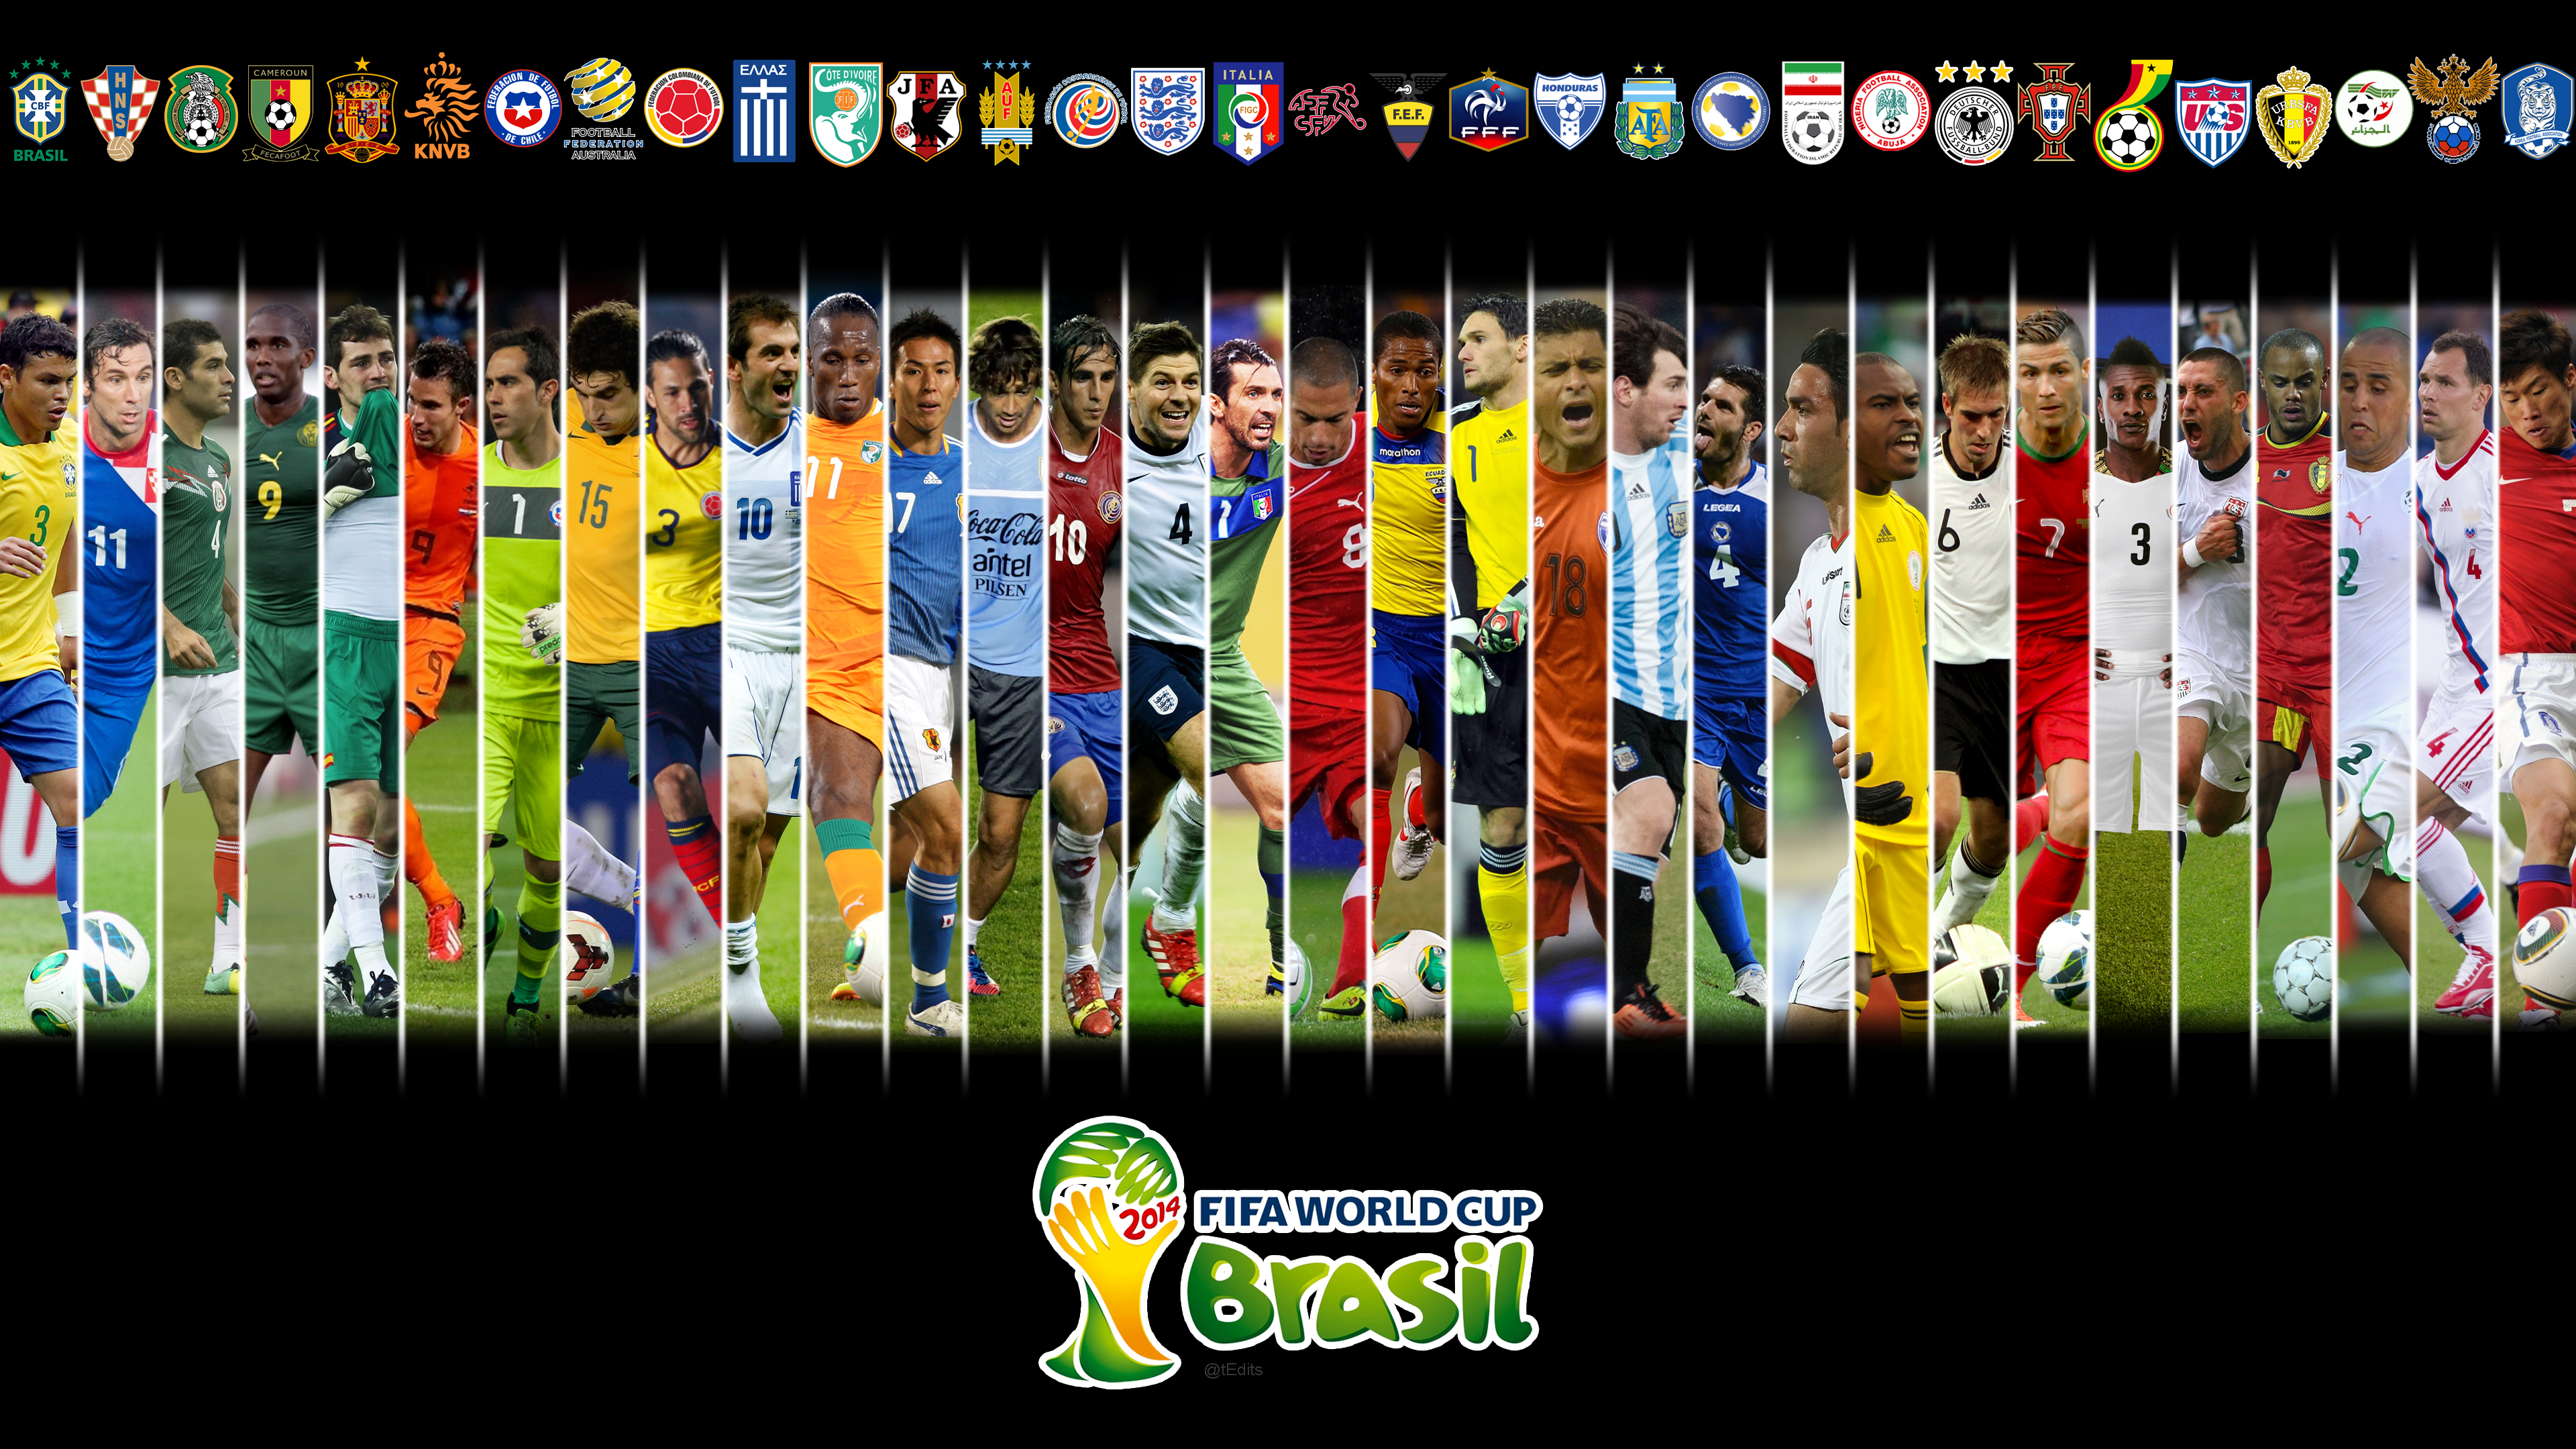
\includegraphics[width=0.8\linewidth]{pic1.png}
\end{figure}

%----------------------------------------------------------------------------------------

\end{column} % End of the first column

\begin{column}{\sepwid}\end{column} % Empty spacer column

\begin{column}{\twocolwid} % Begin a column which is two columns wide (column 2)

\begin{columns}[t,totalwidth=\twocolwid] % Split up the two columns wide column

\begin{column}{\onecolwid}\vspace{-.6in} % The first column within column 2 (column 2.1)

%----------------------------------------------------------------------------------------
%	MATERIALS
%----------------------------------------------------------------------------------------

\begin{block}{Materials}

The following materials were required to complete the research:

\begin{itemize}
\item Bayesian linear regression.
\item Bayesian motivation for proceduralist approach.
\item Probit linear regression.
\item Markov chain Monte Carlo.
\item Gibbs Sampling. 
\end{itemize}

The data were prepared according to the organizations outlined below:

\begin{itemize}
\item FIFA, OPTA, UEFA
\end{itemize}

\end{block}

%----------------------------------------------------------------------------------------

\end{column} % End of column 2.1

\begin{column}{\onecolwid}\vspace{-.6in} % The second column within column 2 (column 2.2)

%----------------------------------------------------------------------------------------
%	METHODS
%----------------------------------------------------------------------------------------

\begin{block}{Model}

We aim to establish the relationship between match results $\boldmath{y} = [y_1, \, y_2, \ldots, y_n]^T \in \mathbb{Z}^n$ and team statistics $\boldmath{X} = [\boldmath{x}_1, \, \boldmath{x}_2, \, \ldots, \boldmath{x}_p ] \in \mathbb{R}^{n \times p}$ whose columns correspond to specific statistics. Since $\boldmath{y}$ is the binary data, we propose to use the following data augmentation approach to model the data: For $i = 1, \, 2, \, \ldots, \, n$, 
\begin{eqnarray}
z_i &\sim& \mathcal{N} (z_i; \, X_i^T \boldmath{\beta}, 1)
\end{eqnarray}
where $z_i$ is the latent variable; $y_i=1 \ if \ z_i>0 \ and \ y_i=0 \ otherwise.$
Moreover, we assign the following prior on $\mathbb{\beta}$:
\begin{eqnarray}
\pi (\boldmath{\beta}) &\sim& \mathcal{N} (\boldmath{\beta}; \boldmath{\beta}_0, \, \Sigma_0 )
\end{eqnarray}
\end{block}

%----------------------------------------------------------------------------------------

\end{column} % End of column 2.2

\end{columns} % End of the split of column 2 - any content after this will now take up 2 columns width

%----------------------------------------------------------------------------------------
%	IMPORTANT RESULT
%----------------------------------------------------------------------------------------

\begin{alertblock}{Important Result}

Among the total 16 elimination matches of 2014 Brazil World Cup, we successfully predict 11 of them, obtaining the accuracy rate of about 70\%.


\end{alertblock} 

%----------------------------------------------------------------------------------------

\begin{columns}[t,totalwidth=\twocolwid] % Split up the two columns wide column again

\begin{column}{\onecolwid} % The first column within column 2 (column 2.1)

%----------------------------------------------------------------------------------------
%	MATHEMATICAL SECTION
%----------------------------------------------------------------------------------------

\begin{block}{Posterior Inference}
The fitted parameters $\hat{\boldmath{\beta}}$ should reflect the corresponding weights for each match statistic. We could employ the fitted $\hat{\boldmath{\beta}}$ to accomplish prediction using new dataset $\tilde{\boldmath{X}}$ as
\begin{equation}
\tilde{\boldmath{z}} = \tilde{\boldmath{X}} \hat{\boldmath{\beta}}
\label{eq:pred}
\end{equation}
\newline
A Gibbs sampler for Bayesian Linear Regression:
\newline \\
\textbf{Sampling} $\boldmath{\beta}$ from
\begin{eqnarray}
(\boldmath{\beta} | -) &\sim& \mathcal{N} ( \boldmath{\beta}; \boldmath{\hat{\beta} }, \, \hat{\Sigma} )
\end{eqnarray}
where
\begin{eqnarray*}
\boldmath{\hat{\beta}} &=& \hat{\Sigma_0} \, ( \Sigma^{-1} \boldmath{\beta_0} + \boldmath{X}^T \boldmath{z} ) \\
\hat{\Sigma} &=& ( \boldmath{X}^T \boldmath{X} + \Sigma_0^{-1} )^{-1}
\end{eqnarray*}
\textbf{Sampling} $z_i$ for $i = 1, \, 2, \, \ldots, \, n$ from
\begin{eqnarray}
(z_i | y_i=0) &\sim& \mathcal{N} ( z_i; X_i^T \boldmath{\beta}, 1 ) \{z_i\leq0\}
\end{eqnarray}
\begin{eqnarray}
(z_i | y_i=1) &\sim& \mathcal{N} ( z_i; X_i^T \boldmath{\beta}, 1 ) \{z_i>0\}
\end{eqnarray}
\end{block}

%----------------------------------------------------------------------------------------

\end{column} % End of column 2.1

\begin{column}{\onecolwid} % The second column within column 2 (column 2.2)

%----------------------------------------------------------------------------------------
%	RESULTS
%----------------------------------------------------------------------------------------

\begin{block}{Results}

\begin{figure}
\includegraphics[width=0.8\linewidth]{Slide3.jpg}
\caption{Prediction Result}
\end{figure}
In the game of Columbia vs Uruguay, Belgium vs USA, France vs Germany, Brazil vs Germany and Brazil vs Netherlands, we did wrong predictions according to the real data. Interestingly, some teams even win the game with the disadvantage in all fields.

\begin{table}
\vspace{0ex}
\begin{tabular}{l l l}
\toprule
\textbf{Correct} & \textbf{Wrong} & \textbf{Accuracy}\\
\midrule
11 & 5 & 68.75\% \\
\bottomrule
\end{tabular}
\caption{Prediction Outcome}
\end{table}

\end{block}

%----------------------------------------------------------------------------------------

\end{column} % End of column 2.2

\end{columns} % End of the split of column 2

\end{column} % End of the second column

\begin{column}{\sepwid}\end{column} % Empty spacer column

\begin{column}{\onecolwid} % The third column

%----------------------------------------------------------------------------------------
%	CONCLUSION
%----------------------------------------------------------------------------------------

\begin{block}{Conclusion}

This model introduces latent parameter for making prediction. In our model, we establish the relationship between match statistics in each soccer team and the result of a match. For our method, we implement the Gibbs sampling to perform the posterior inference. The experimental results tell us that the models can fit the data well and provide the reasonable prediction.

\end{block}

%----------------------------------------------------------------------------------------
%	ADDITIONAL INFORMATION
%----------------------------------------------------------------------------------------

\begin{block}{Additional Information}

Further, we plan to apply some non-linear algorithms to make the prediction, like 
\begin{itemize}
\item Non-linear SVM
\item Gaussian process regression
\end{itemize}

\end{block}

%----------------------------------------------------------------------------------------
%	REFERENCES
%----------------------------------------------------------------------------------------

\begin{block}{References}
\begin{thebibliography}{99}
\bibitem{ref1} Alexander Spermann. \textit{The Probit Model, University of Freiburg}. Sose, 2009.
\bibitem{ref2} Peter D Hoff. \textit{A first course in Bayesian statistical methods}. Springer, 2009.
\end{thebibliography}
\end{block}

%----------------------------------------------------------------------------------------
%	ACKNOWLEDGEMENTS
%----------------------------------------------------------------------------------------

\setbeamercolor{block title}{fg=red,bg=white} % Change the block title color

\begin{block}{Acknowledgements}

\small{\rmfamily{We would like to express our special thanks of gratitude to our instructor (Sayan Mukherjee) who gave us the opportunity to do this interesting project of the World Cup topic, which also helped us doing a lot of research and we came to know about so much more.}} \\

\end{block}

%----------------------------------------------------------------------------------------
%	CONTACT INFORMATION
%----------------------------------------------------------------------------------------

\setbeamercolor{block alerted title}{fg=black,bg=norange} % Change the alert block title colors
\setbeamercolor{block alerted body}{fg=black,bg=white} % Change the alert block body colors

\begin{alertblock}{Contact Information}

\begin{itemize}
\item Web: \href{http://www.ece.duke.edu}{http://www.ece.duke.edu}
\item Email: \href{mailto:wen.bo@duke.edu}{wen.bo@duke.edu}
\item Phone: +1 (919) 808 7710 
\end{itemize}

\end{alertblock}

\begin{center}
\begin{tabular}{ccc}
%\includegraphics[width=0.4\linewidth]{logo.png} & \hfill & \includegraphics[width=0.4\linewidth]{logo.png}
\includegraphics[width=0.6\linewidth]{pic4.jpg} 
\end{tabular}
\end{center}

%----------------------------------------------------------------------------------------

\end{column} % End of the third column

\end{columns} % End of all the columns in the poster

\end{frame} % End of the enclosing frame

\end{document}
